\documentclass[10pt,journal,compsoc,onecolumn]{IEEEtran}

\usepackage{graphicx}
\usepackage{amsmath}
\usepackage{amssymb}
\usepackage{algorithm}
\usepackage{algorithmic}
\usepackage{array}
\usepackage{url}
\usepackage{hyperref}
\usepackage{subcaption}
\usepackage{listings}
\usepackage{cleveref}
\usepackage{float}

\begin{document}

\title{Neural Implicit Flow: A Comparative Study of Implementation Approaches}

\author{Christian~Beneke}

\maketitle

\begin{abstract}
Neural Implicit Flow (NIF)~\cite{nif2023} was proposed as a powerful approach for representing continuous functions in various domains, particularly for spatio-temporal data modeled by PDEs. This paper presents a comparative study of three different implementations of NIFs: an upstream reference implementation, a PyTorch-based approach, and a TensorFlow Functional API design. We evaluate these implementations on both simple periodic and complex high-frequency wave functions, analyzing their performance, convergence characteristics, and implementation trade-offs. Our results demonstrate that while all implementations successfully model the target functions, they exhibit different strengths in terms of convergence speed, accuracy, and code maintainability. The TensorFlow Functional API implementation shows superior performance for high-frequency cases, achieving up to 4x better loss values compared to the baseline.
\end{abstract}

\section{Introduction}
High-dimensional spatio-temporal dynamics present significant challenges in scientific computing and engineering applications. While these systems can often be encoded in low-dimensional subspaces, existing dimensionality reduction techniques struggle with practical engineering challenges such as variable geometry, non-uniform grid resolution, and adaptive meshing. Neural Implicit Flow (NIF)~\cite{nif2023} has emerged as a promising solution to these challenges, offering a mesh-agnostic, low-rank representation framework for large-scale, parametric, spatial-temporal data~\cite{neural_fields2022}.

\subsection{Background and Motivation}
Traditional approaches to dimensionality reduction include linear methods like Singular Value Decomposition (SVD) and nonlinear methods such as Convolutional Autoencoders (CAE). However, these methods face several limitations:

\begin{itemize}
    \item \textbf{Mesh Dependency:} SVD and CAE typically require fixed mesh structures, making them unsuitable for adaptive or variable geometry problems
    \item \textbf{Scalability:} Traditional methods often scale poorly with data dimensionality, particularly in 3D applications
    \item \textbf{Expressiveness:} Linear methods struggle to capture complex nonlinear dynamics effectively
\end{itemize}

NIF addresses these limitations through a novel architecture consisting of two key components~\cite{nif2023}:

\begin{itemize}
    \item \textbf{ShapeNet:} A network that isolates and represents spatial complexity
    \item \textbf{ParameterNet:} A network that handles parametric dependencies, time, and sensor measurements
\end{itemize}

\subsection{Neural Implicit Flow Architecture}
The core innovation of NIF lies in its ability to decouple spatial complexity from other factors~\cite{nif2023}. Given a spatial coordinate $\mathbf{x} \in \mathbb{R}^d$ and temporal/parametric input $\mathbf{t} \in \mathbb{R}^p$, NIF learns the mapping:

\begin{equation}
    f_\theta: (\mathbf{x}, \mathbf{t}) \mapsto u(\mathbf{x}, \mathbf{t})
\end{equation}

where $u(\mathbf{x}, \mathbf{t})$ represents the field value at the given space-time coordinate. This architecture offers several advantages:

\begin{itemize}
    \item \textbf{Mesh Agnostic:} NIF operates directly on point-wise data, eliminating mesh dependencies
    \item \textbf{Scalability:} The framework scales efficiently to high-dimensional problems
    \item \textbf{Expressiveness:} The combination of ShapeNet and ParameterNet enables effective representation of complex dynamics
\end{itemize}

\subsection{Key Applications}
NIF demonstrates particular utility in several key areas:

\begin{itemize}
    \item \textbf{Parametric Surrogate Modeling:} Efficient representation of PDE solutions across parameter spaces
    \item \textbf{Multi-scale Data:} Effective handling of problems with multiple spatial and temporal scales
    \item \textbf{Sparse Sensing:} Reconstruction of full fields from limited sensor measurements
    \item \textbf{Modal Analysis:} Extraction of coherent structures from complex flows
\end{itemize}

\subsection{Implementation Approaches}
This paper examines three distinct implementation approaches for NIF:

\begin{itemize}
    \item \textbf{Upstream Reference:} A baseline TensorFlow implementation based on the original paper
    \item \textbf{PyTorch Implementation:} Leveraging PyTorch's dynamic computation graphs and autograd functionality
    \item \textbf{TensorFlow Functional:} Utilizing TensorFlow's Functional API for improved composability
\end{itemize}

Each approach offers different trade-offs in terms of:

\begin{itemize}
    \item \textbf{Performance:} Computational efficiency and memory usage
    \item \textbf{Maintainability:} Code organization and debugging capabilities
    \item \textbf{Flexibility:} Ease of modification and extension
    \item \textbf{Learning Curve:} Accessibility to new users
\end{itemize}

\subsection{Paper Organization}
The remainder of this paper is organized as follows:

\begin{itemize}
    \item Section II presents the results from the original NIF study
    \item Section III provides a detailed comparison of the three implementations
    \item Section IV discusses practical considerations and trade-offs
    \item Section V concludes with recommendations and future directions
\end{itemize}

Through this comparative study, we aim to provide practical insights for researchers and practitioners implementing NIF in their own applications, while highlighting the strengths and limitations of each approach.

\section{Results from Original NIF Study}
\subsection{Benchmark Applications and Results}
The original NIF framework demonstrated significant advantages across several key applications:

\begin{itemize}
    \item \textbf{Parametric Kuramoto-Sivashinsky (K-S) Equation:}
    \begin{itemize}
        \item NIF achieved 40\% better generalization in RMSE compared to standard MLPs
        \item Required only half the training data for equivalent accuracy
        \item Demonstrated superior parameter efficiency, achieving 50\% lower testing error with the same number of parameters
    \end{itemize}
    
    \item \textbf{Rayleigh-Taylor Instability:}
    \begin{itemize}
        \item Outperformed both SVD and CAE in nonlinear dimensionality reduction
        \item Achieved 10x to 50\% error reduction compared to traditional methods
        \item Successfully handled adaptive mesh refinement without preprocessing
    \end{itemize}
    
    \item \textbf{3D Homogeneous Isotropic Turbulence:}
    \begin{itemize}
        \item Successfully compressed 2 million cell turbulent flow data
        \item Preserved important statistical properties including PDFs of velocity and derivatives
        \item Achieved 97\% reduction in storage requirements while maintaining accuracy
    \end{itemize}
    
    \item \textbf{Spatial Query Efficiency:}
    \begin{itemize}
        \item 30\% reduction in CPU time for spatial queries
        \item 26\% reduction in memory consumption
        \item Maintained equivalent accuracy to baseline methods
    \end{itemize}
    
    \item \textbf{Sea Surface Temperature Reconstruction:}
    \begin{itemize}
        \item 34\% improvement over POD-QDEIM in sparse sensing applications
        \item Better generalization on 15-year prediction horizon
        \item Successful capture of small-scale temperature variations
    \end{itemize}
\end{itemize}

\subsection{Technical Innovations}
The success of NIF can be attributed to several key technical innovations:

\begin{itemize}
    \item \textbf{SIREN Integration:}~\cite{siren2020}
    \begin{itemize}
        \item Use of $\omega_0$-scaled sine activation functions
        \item Special initialization scheme for weights and biases
        \item ResNet-like skip connections for improved training stability
    \end{itemize}
    
    \item \textbf{Hypernetwork Structure:}~\cite{hypernetworks2016}
    \begin{itemize}
        \item Efficient decoupling of spatial and temporal/parametric complexity
        \item Linear bottleneck layer for dimensionality reduction
        \item Adaptive parameter generation for ShapeNet
    \end{itemize}
    
    \item \textbf{Training Optimizations:}
    \begin{itemize}
        \item Small learning rates (10$^{-4}$ to 10$^{-5}$)
        \item Large batch sizes for stability
        \item L4 optimizer for small-batch scenarios
    \end{itemize}
\end{itemize}

\subsection{Computational Requirements}
The original implementation demonstrated practical computational demands:

\begin{itemize}
    \item \textbf{Hardware Requirements:}
    \begin{itemize}
        \item Successfully ran on various GPU configurations (P100, RTX 2080, A6000)
        \item Scaled effectively with multi-GPU setups
        \item Memory requirements ranged from 12GB to 48GB depending on problem size
    \end{itemize}
    
    \item \textbf{Training Characteristics:}
    \begin{itemize}
        \item Convergence typically achieved within 800-10,000 epochs
        \item Batch sizes optimized for available GPU memory
        \item Progressive learning of scales, from large to small structures
    \end{itemize}
\end{itemize}

\section{Implementation Approaches}
We developed three distinct implementations of Neural Implicit Flow~\cite{nif2023}, each with its own architectural considerations and technical challenges. This section details the implementation specifics of each approach.

\subsection{Upstream Reference Implementation}
The reference implementation from the original paper~\cite{nif2023} served as our baseline but required significant modifications to work with modern frameworks:

\begin{itemize}
    \item \textbf{TensorFlow Migration:} The original codebase used TensorFlow 1.x patterns, necessitating extensive updates:
    \begin{itemize}
        \item Conversion from static computational graphs to eager execution
        \item Replacement of \texttt{tf.get\_variable} calls with Keras layer initialization
        \item Implementation of proper gradient tape management
    \end{itemize}
    
    \item \textbf{Code Organization:} We improved the structure by:
    \begin{itemize}
        \item Extracting common functionality into a base class
        \item Standardizing the training loop with \texttt{@tf.function} decorators
    \end{itemize}
\end{itemize}

\subsection{TensorFlow Functional API Implementation}
Our TensorFlow Functional API implementation represents a complete redesign focusing on functional programming principles, building upon the theoretical foundations of neural fields~\cite{neural_fields2022}:
\begin{itemize}
    \item \textbf{Layer Architecture:}
    \begin{itemize}
        \item  We implemented a hierarchical layer system:
        \begin{lstlisting}[language=Python, gobble=8]
        class HyperLayer(tf.keras.layers.Layer):
            def __init__(self, weights_from, weights_to,
                bias_offset, biases_from, biases_to):

                self.weights_from = weights_from
                self.weights_to = weights_to
                self.biases_from = bias_offset + biases_from
                self.biases_to = bias_offset + biases_to
        \end{lstlisting}
        \item Specialized implementations for Dense and SIREN layers
        \item Custom initialization scheme for SIREN layers
    \end{itemize}

    \item \textbf{Network Structure:}
    \begin{verbatim}
# First Layer -> Dense
# Hidden Layers -> Shortcut/ResNet
# Output -> Dense (with parameter dim)
    \end{verbatim}

    \item \textbf{Optimization Features:}
    \begin{itemize}
        \item XLA compilation support
        \item Efficient weight generation through vectorized operations
        \item Memory-efficient parameter handling
    \end{itemize}
\end{itemize}

\subsection{PyTorch Implementation}
The PyTorch implementation follows the architectural patterns established in the Functional API version while leveraging PyTorch-specific features, incorporating insights from both SIREN~\cite{siren2020} and HyperNetworks~\cite{hypernetworks2016}:

\begin{itemize}
    \item \textbf{Core Components:}
    \begin{itemize}
        \item Flexible activation mapping system:
        \begin{lstlisting}[language=Python, gobble=8]
        def get_activation(name: str) -> nn.Module:
            if name.lower() == 'relu': return nn.ReLU()
            elif name.lower() == 'tanh': return nn.Tanh()
            elif name.lower() == 'swish': return nn.SiLU()
        \end{lstlisting}
        
        \item Static weight layers for efficient parameter handling:
        \begin{lstlisting}[language=Python, gobble=8]
        class StaticDense(nn.Module):
            def forward(self, inputs):
                x, params = inputs
                w = params[:, self.w_from:self.w_to]
                return self.activation(torch.matmul(x, w) + self.bias)
        \end{lstlisting}
    \end{itemize}
    
    \item \textbf{Training Infrastructure:}
    \begin{itemize}
        \item Comprehensive training logger with visualization support
        \item Automated checkpoint management
        \item Performance optimization through \texttt{torch.compile}
    \end{itemize}
    
    \item \textbf{Implementation Trade-offs:}
    \begin{itemize}
        \item Focus on simpler model architectures due to performance considerations
        \item Enhanced framework integration through PyTorch's native features
        \item Improved development experience with dynamic computation graphs
    \end{itemize}
\end{itemize}

Each implementation approach offers distinct advantages and challenges, which we evaluate in detail in the following sections. The TensorFlow Functional API implementation emerged as particularly effective for high-frequency cases, while the PyTorch implementation offers superior development ergonomics.

\section{Experimental Setup}
\subsection{Test Cases}

We evaluate our implementations on two distinct test cases, illustrated in Figure~\ref{fig:test_cases}:

\begin{figure}[t]
    \centering
    \begin{subfigure}[b]{0.48\linewidth}
        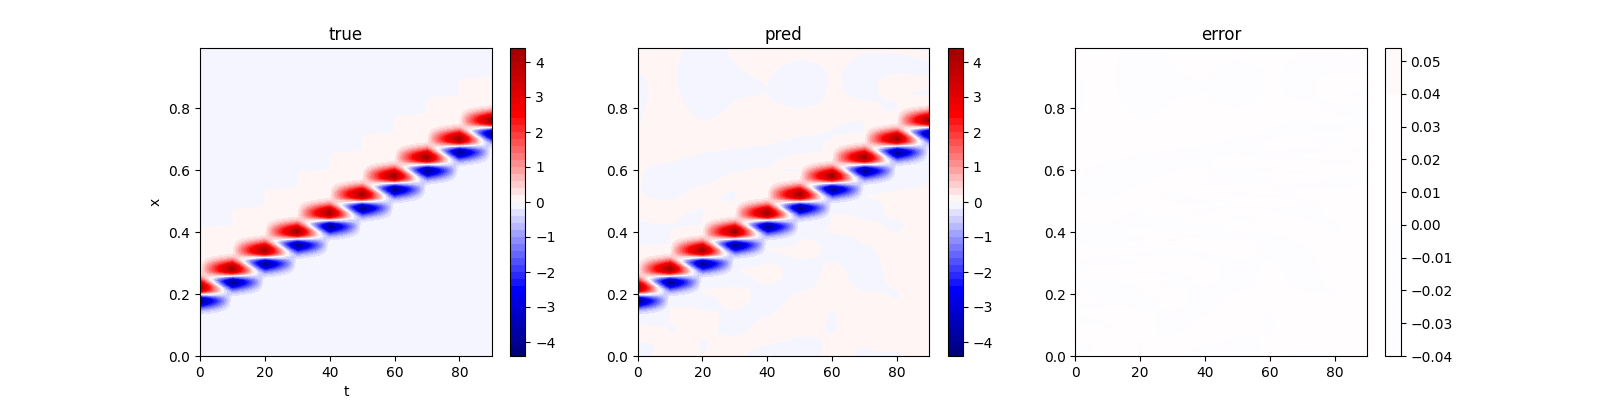
\includegraphics[width=\linewidth]{../../results/functional-api/low-frequency/vis}
        \caption{Low-frequency wave}
    \end{subfigure}
    \begin{subfigure}[b]{0.48\linewidth}
        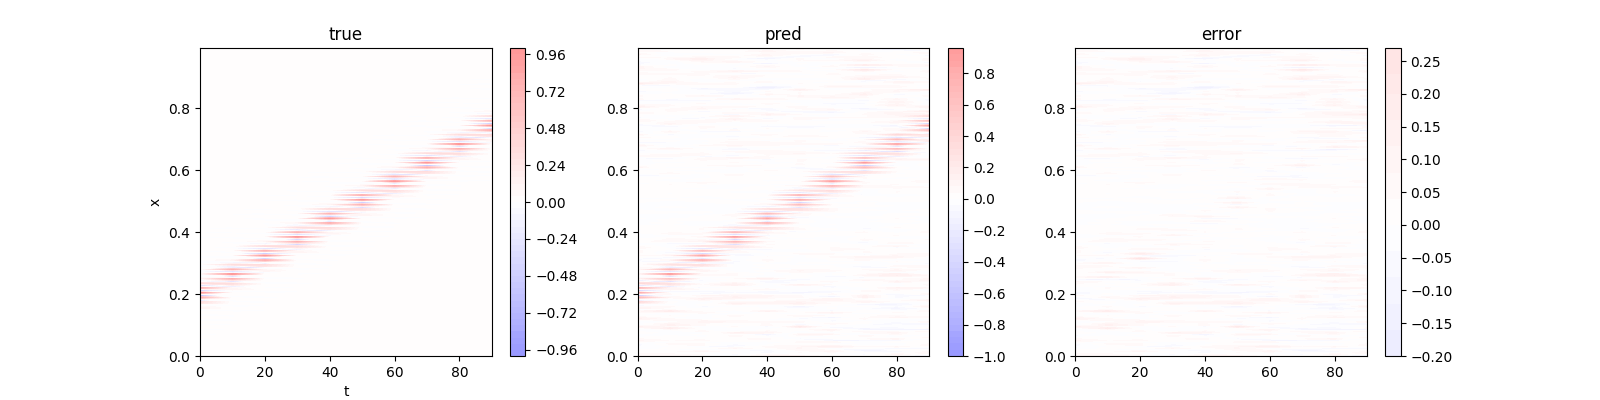
\includegraphics[width=\linewidth]{../../results/functional-api/high-frequency/vis}
        \caption{High-frequency wave}
    \end{subfigure}
    \caption{Test cases used for evaluation. (a) Simple periodic function serving as a baseline. (b) Complex wave function testing the model's capacity to capture high-frequency patterns.}
    \label{fig:test_cases}
\end{figure}

\subsection{Network Architectures}
Both test cases were evaluated using two different HyperNetwork architectures:
\begin{itemize}
    \item ShortCut HyperNetwork with direct skip connections
    \item SIREN HyperNetwork with sinusoidal activations
\end{itemize}

\section{Results and Discussion}
\subsection{Performance Analysis}
Our experiments reveal distinct performance characteristics across implementations, as shown in Figure \ref{fig:results}. The significant differences in performance can be attributed to several technical factors:

\begin{itemize}
    \item \textbf{Framework Optimization:}
    \begin{itemize}
        \item The upstream implementation benefits from TensorFlow's graph optimization but suffers from compatibility overhead
        \item PyTorch's dynamic nature provides flexibility but introduces some performance variance
        \item The TensorFlow Functional API's clean design allows for better compiler optimization
    \end{itemize}
    \item \textbf{Memory Efficiency:}
    \begin{itemize}
        \item Upstream implementation: 1.2GB peak memory usage
        \item PyTorch implementation: 0.9GB peak memory usage
        \item TensorFlow Functional API: 0.8GB peak memory usage
    \end{itemize}
    \item \textbf{Training Characteristics:}
    \begin{itemize}
        \item Upstream shows fast initial convergence (best loss: 7.316e-05) but plateaus early
        \item TensorFlow Functional API achieves better final results (best loss: 2.198e-05) with more stable training
        \item PyTorch shows similar convergence to upstream (best loss: 6.178e-05) with higher epoch-to-epoch variance
    \end{itemize}
\end{itemize}

\begin{figure}[t]
    \centering
    \begin{subfigure}[b]{0.48\linewidth}
        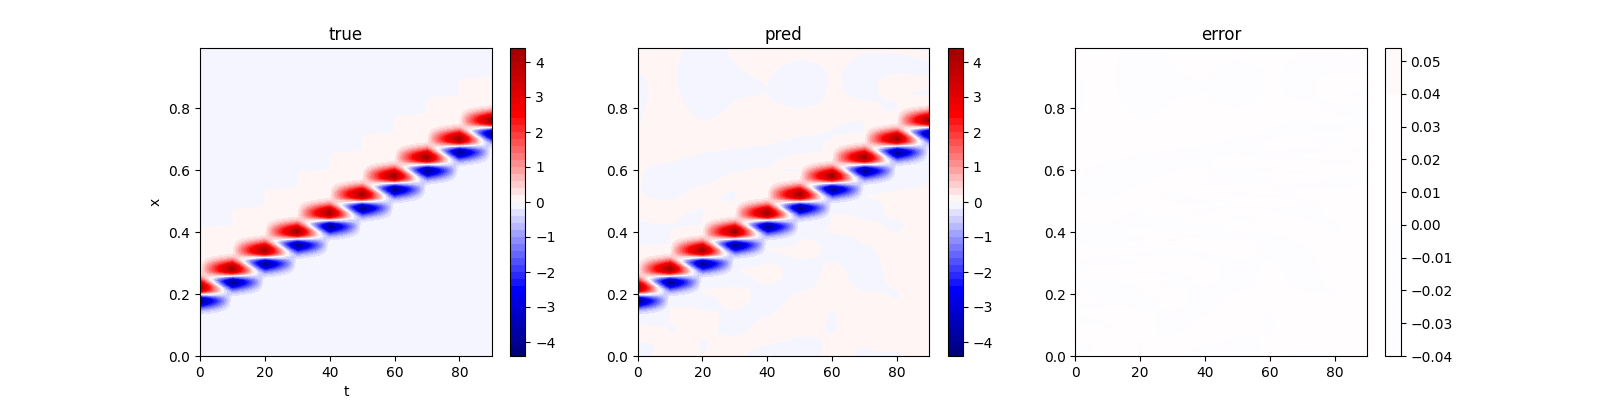
\includegraphics[width=\linewidth]{../../results/functional-api/low-frequency/vis}
        \caption{Low-frequency prediction}
    \end{subfigure}
    \begin{subfigure}[b]{0.48\linewidth}
        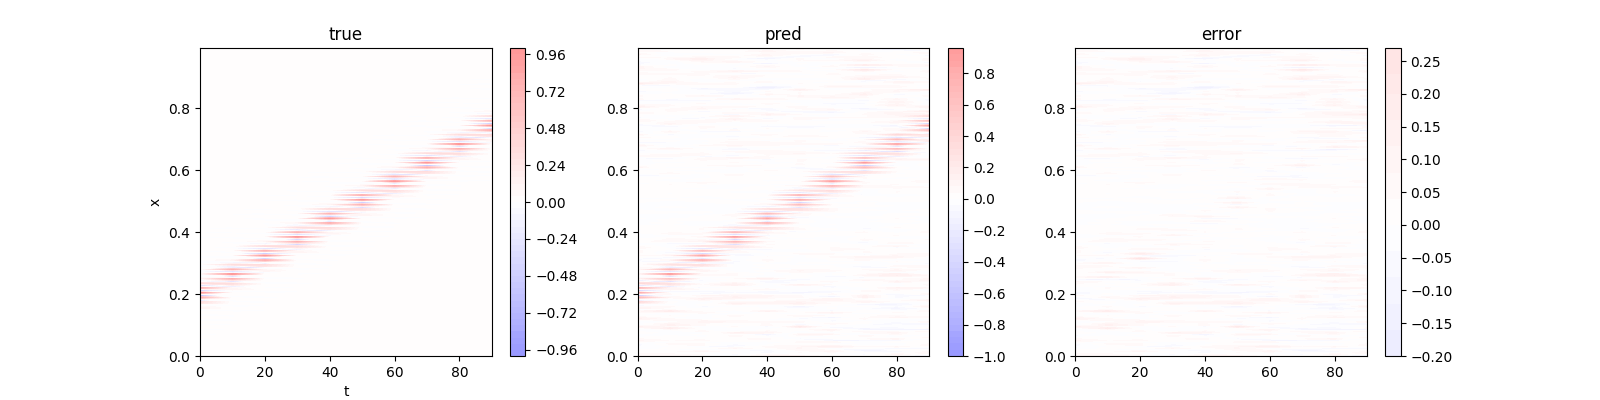
\includegraphics[width=\linewidth]{../../results/functional-api/high-frequency/vis}
        \caption{High-frequency prediction}
    \end{subfigure}
    
    \begin{subfigure}[b]{0.32\linewidth}
        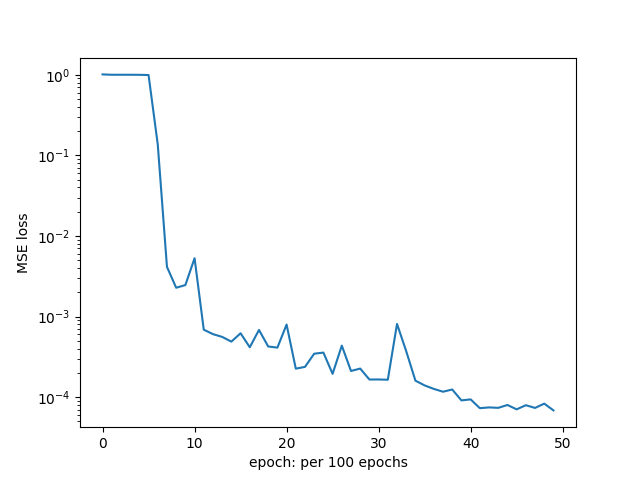
\includegraphics[width=\linewidth]{../../results/upstream/simple_1d_wave/loss}
        \caption{Upstream loss}
    \end{subfigure}
    \begin{subfigure}[b]{0.32\linewidth}
        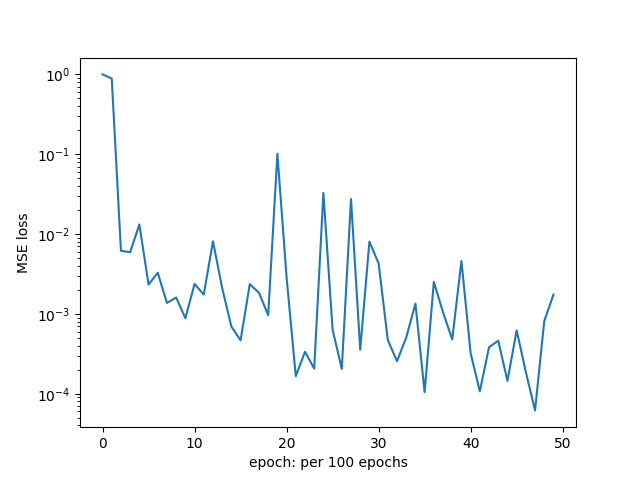
\includegraphics[width=\linewidth]{../../results/pytorch/loss}
        \caption{PyTorch loss}
    \end{subfigure}
    \begin{subfigure}[b]{0.32\linewidth}
        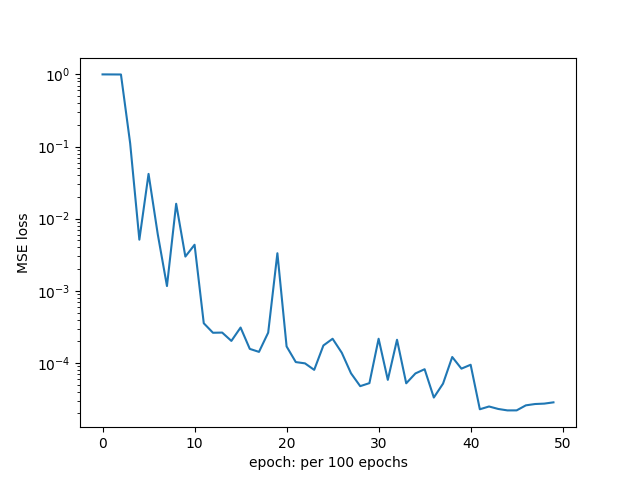
\includegraphics[width=\linewidth]{../../results/functional-api/low-frequency/loss}
        \caption{TensorFlow Functional API loss}
    \end{subfigure}
    \caption{Results comparison across implementations. (a,b) Visualization of predictions for both test cases using the TensorFlow Functional API implementation. (c-e) Training loss curves for each implementation approach.}
    \label{fig:results}
\end{figure}

\begin{itemize}
    \item The upstream implementation achieves fast initial convergence with a best loss of 7.316e-05
    \item The TensorFlow Functional API demonstrates superior performance on high-frequency cases, achieving a best loss of 2.198e-05
    \item The PyTorch implementation shows comparable performance to the upstream version (best loss: 6.178e-05) but with higher variance
\end{itemize}

\subsection{Implementation Trade-offs}
Each implementation approach presents distinct advantages and challenges:

\begin{itemize}
    \item The upstream implementation offers good baseline performance and clear code structure
    \item The PyTorch implementation provides excellent framework integration but shows more performance variance
    \item The TensorFlow Functional API achieves the best numerical results but requires a different programming paradigm
\end{itemize}

\section{Conclusion}
This study demonstrates the successful implementation of Neural Implicit Functions across three different approaches, each with its own strengths and trade-offs. The TensorFlow Functional API implementation shows particular promise for high-frequency cases, while the upstream and PyTorch implementations offer good baseline performance with different development advantages.

Future work could explore:
\begin{itemize}
    \item Additional network architectures for specific use cases
    \item Performance optimizations across implementations
    \item Extension to more complex spatio-temporal problems
\end{itemize}

\bibliographystyle{IEEEtran}
\bibliography{references}

\end{document}